\documentclass[a4paper, 11pt]{article}
\usepackage{comment} % enables the use of multi-line comments (\ifx \fi) 
\usepackage{lipsum} %This package just generates Lorem Ipsum filler text. 
\usepackage{fullpage} % changes the margin
\usepackage[a4paper, total={7in, 10in}]{geometry}
\usepackage[fleqn]{amsmath}
\usepackage{amssymb,amsthm}  % assumes amsmath package installed
\newtheorem{theorem}{Theorem}
\newtheorem{corollary}{Corollary}
\usepackage{graphicx}
\usepackage{tikz}
\usetikzlibrary{arrows}
\usepackage{verbatim}
\usepackage[numbered]{mcode}
\usepackage{float}
\usepackage{subcaption}
\usepackage{tikz}
    \usetikzlibrary{shapes,arrows}
    \usetikzlibrary{arrows,calc,positioning}

    \tikzset{
        block/.style = {draw, rectangle,
            minimum height=1cm,
            minimum width=1.5cm},
        input/.style = {coordinate,node distance=1cm},
        output/.style = {coordinate,node distance=4cm},
        arrow/.style={draw, -latex,node distance=2cm},
        pinstyle/.style = {pin edge={latex-, black,node distance=2cm}},
        sum/.style = {draw, circle, node distance=1cm},
    }
\usepackage{xcolor}
\usepackage{mdframed}
\usepackage[shortlabels]{enumitem}
\usepackage{indentfirst}
\usepackage{hyperref}
    
\renewcommand{\thesubsection}{\thesection.\alph{subsection}}

\newenvironment{problem}[2][Problem]
    { \begin{mdframed}[backgroundcolor=gray!20] \textbf{#1 #2} \\}
    {  \end{mdframed}}

% Define solution environment
\newenvironment{solution}
    {\textit{Solution:}}
    {}

\renewcommand{\qed}{\quad\qedsymbol}
%%%%%%%%%%%%%%%%%%%%%%%%%%%%%%%%%%%%%%%%%%%%%%%%%%%%%%%%%%%%%%%%%%%%%%%%%%%%%%%%%%%%%%%%%%%%%%%%%%%%%%%%%%%%%%%%%%%%%%%%%%%%%%%%%%%%%%%%
\begin{document}
%Header-Make sure you update this information!!!!
\noindent
%%%%%%%%%%%%%%%%%%%%%%%%%%%%%%%%%%%%%%%%%%%%%%%%%%%%%%%%%%%%%%%%%%%%%%%%%%%%%%%%%%%%%%%%%%%%%%%%%%%%%%%%%%%%%%%%%%%%%%%%%%%%%%%%%%%%%%%%
\large\textbf{Mengke Li} \hfill \textbf{Homework - \#4}   \\
Email: mengkel@clemson.edu \hfill ID: C28207748 \\
\normalsize Course: CPSC 8430 - Deep Learning \hfill Term: Spring 2023\\
Instructor: Dr. Luo \hfill Due Date: $22^{nd}$ April, 2023 \\
Github Link: https://github.com/mengkel/CPSC-8430-DP-HW/tree/main/HW4 \\
\noindent\rule{7in}{2.8pt}
%%%%%%%%%%%%%%%%%%%%%%%%%%%%%%%%%%%%%%%%%%%%%%%%%%%%%%%%%%%%%%%%%%%%%%%%%%%%%%%%%%%%%%%%%%%%%%%%%%%%%%%%%%%%%%%%%%%%%%%%%%%%%%%%%%%%%%%%
% Problem 1
%%%%%%%%%%%%%%%%%%%%%%%%%%%%%%%%%%%%%%%%%%%%%%%%%%%%%%%%%%%%%%%%%%%%%%%%%%%%%%%%%%%%%%%%%%%%%%%%%%%%%%%%%%%%%%%%%%%%%%%%%%%%%%%%%%%%%%%%
\begin{problem}{1-1: Train a Discriminator/Generator pair on CIFAR10 dataset utilizing techniques from DCGAN, Wasserstein GANs,
ACGAN}
\end{problem}
\begin{itemize}
\item First, I will have a brief introduction of DCGAN and WGAN and their difference.
DCGAN means Deep Convolutional Generative Adversarial Network and WGAN stands for Wasserstein Generative Adversarial Network. The difference of those two algrithm are:

\item[1]
DCGAN uses the sigmoid activation function in the output layer of the discriminator to predict the likelihood of a given image being real. WGAN uses a linear activation function in the output layer of the critic model.
\item[2]
DCGAN uses 1 nad 0 as the labels as the real and fake images. while WGAN uses -1 labels for real images and 1 labels for fake images.
\item[3]

The DCGAN trains the discriminator as a binary classification model to predict the probability that a given image is real. Therefore, the discriminator is optimized using the binary cross entropy loss function. The same loss function is used to update the generator model.

WGAN model uses a new loss function that encourages the discriminator to predict a score of how real or fake a given input looks.

\item[4]
The DCGAN does not use any gradient clipping, although the WGAN requires gradient clipping for the critic model.

\item[5]
DCGAN update the discriminator and generator in equal amounts. 
WGAN updates the critic model more times than the generator each iteration (e.g. 5).

\end{itemize}

\begin{solution}

\begin{itemize}
\item The training data examples
\begin{figure}[H]
\centering    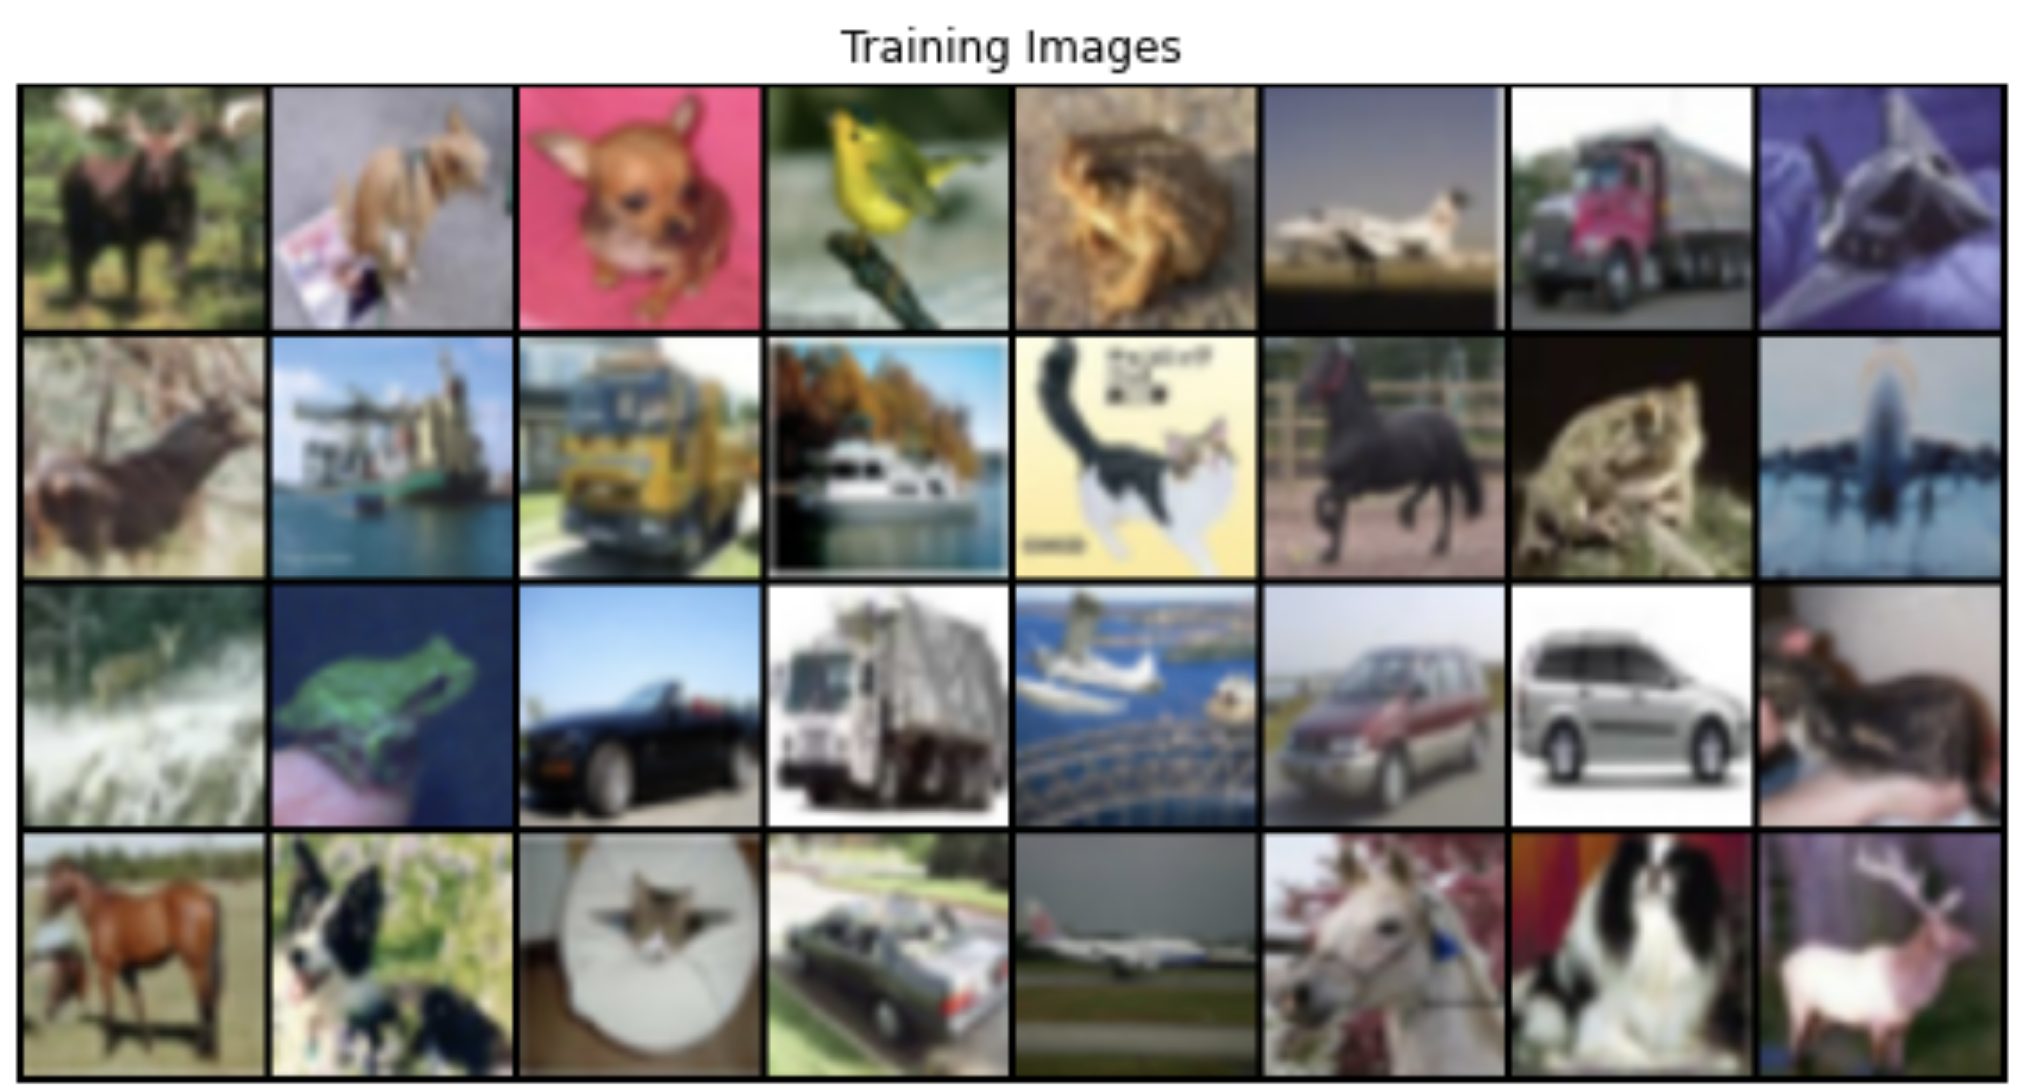
\includegraphics[scale=0.4]{example.png}
    \label{fig:1-1}
\end{figure}

\item The training loss for generator and discriminator in the DCGAN model.
\begin{figure}[H]
\centering    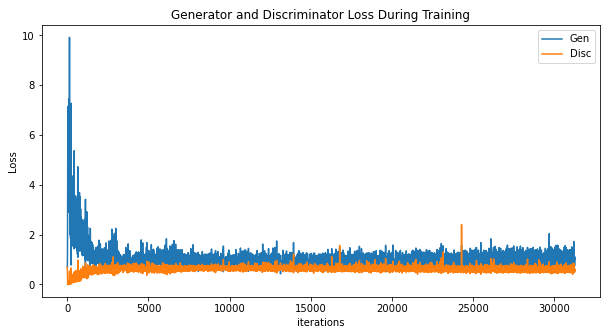
\includegraphics[scale=0.6]{DCGAN-loss.png}
    \label{fig:1-2}
\end{figure}

\item The comparison of real image and fake image generated by the trained generator in DCGAN.

\begin{figure}[H]
\centering    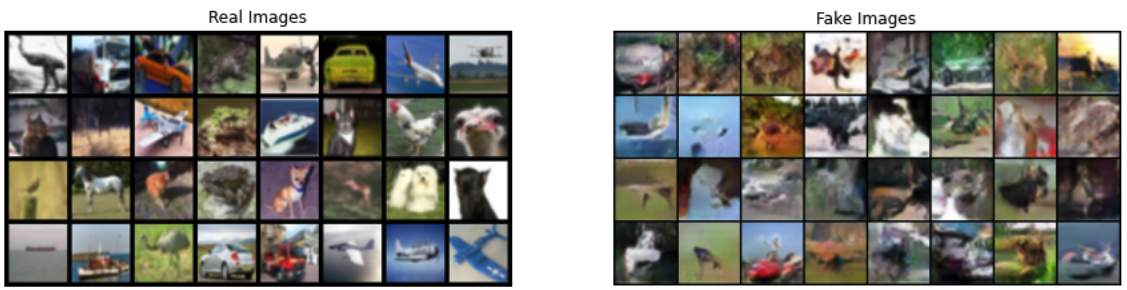
\includegraphics[scale=0.4]{DC-GAN-compare.png}
    \label{fig:1-3}
\end{figure}


\item The training loss for generator and discriminator in WGAN model.
\begin{figure}[H]
\centering    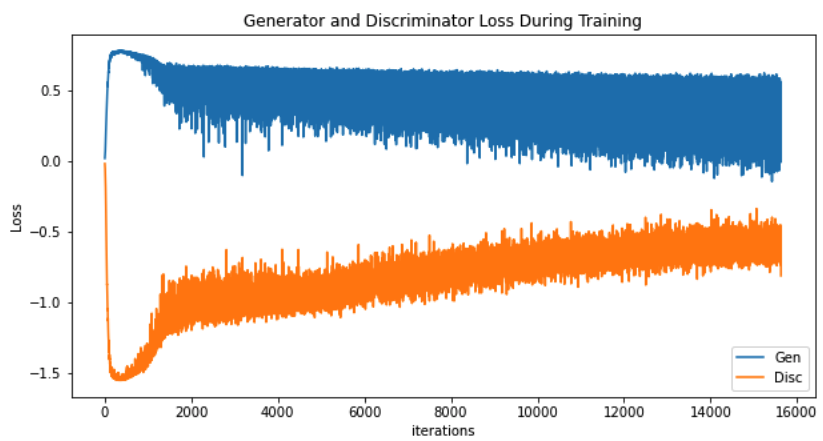
\includegraphics[scale=0.5]{W-GAN-loss.png}
    \label{fig:1-4}
\end{figure}

\item The comparison of real image and fake image generated by the trained generator in WGAN model.

\begin{figure}[H]
\centering    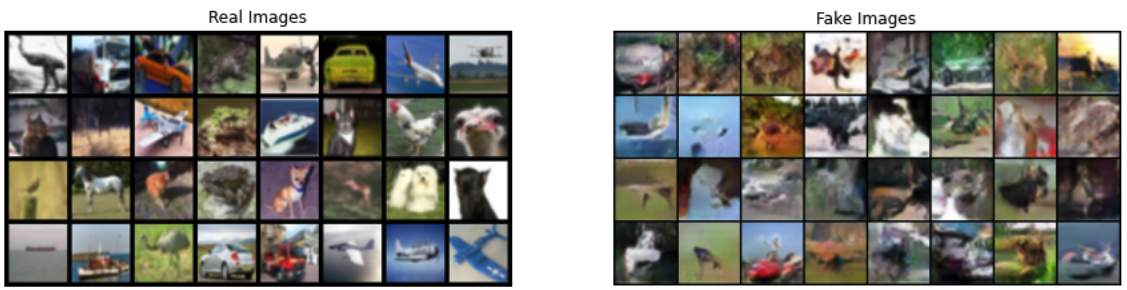
\includegraphics[scale=0.43]{DC-GAN-compare.png}
    \label{fig:1-5}
\end{figure}

\item The comparison of the fretchet distances in DC-GAN and W-GAN models.

\begin{figure}[H]
\centering    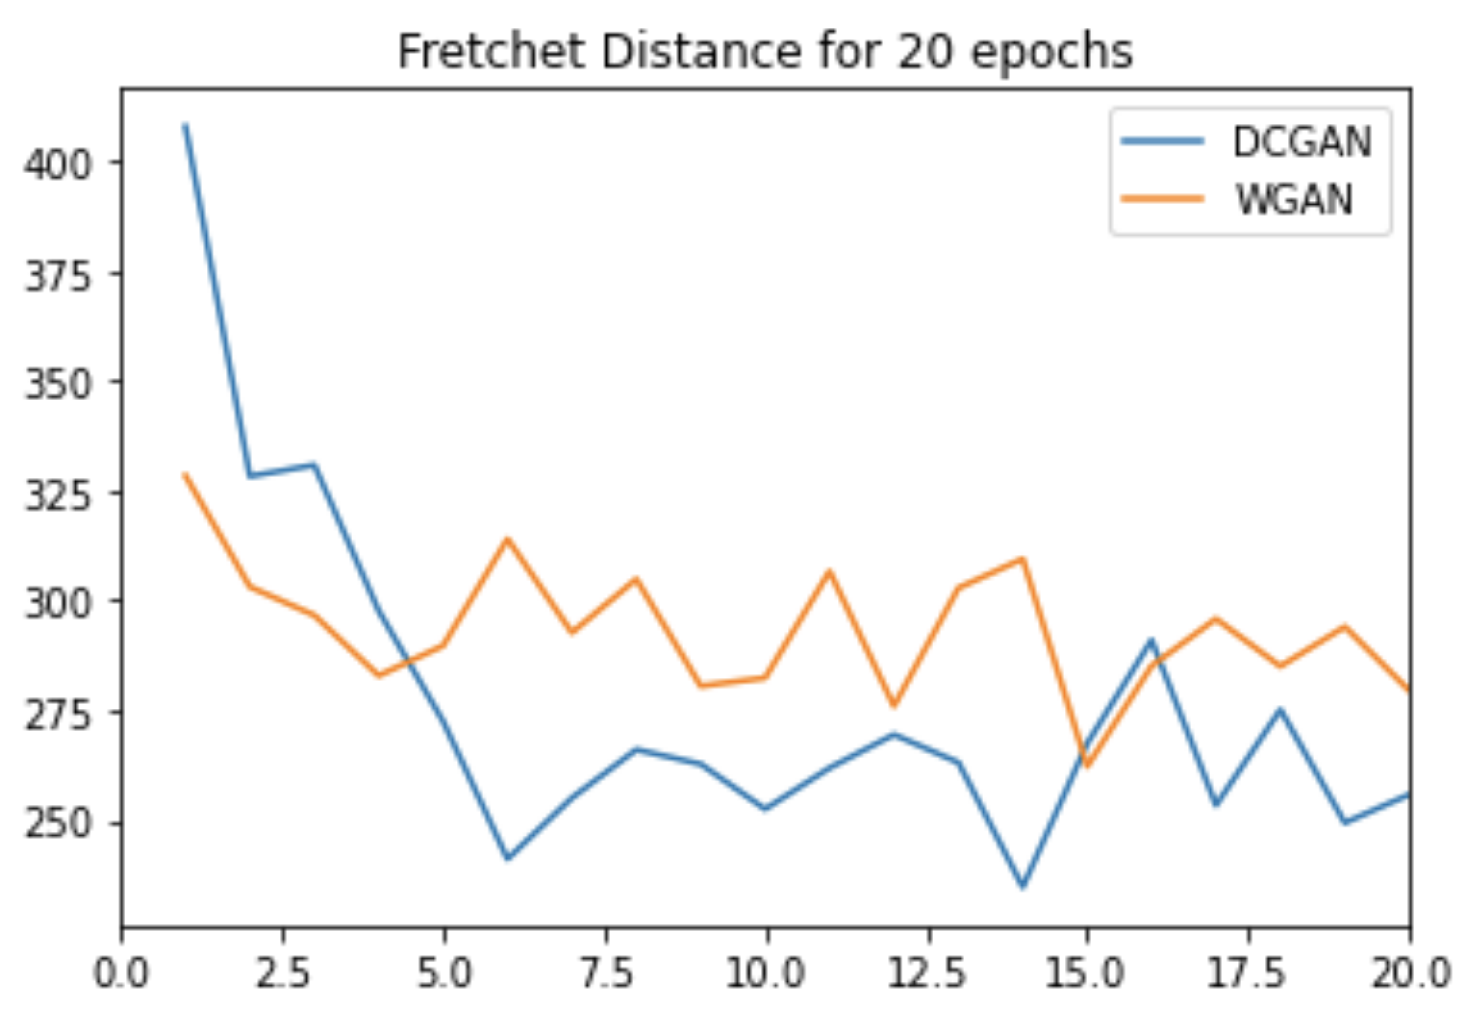
\includegraphics[scale=0.43]{fd.png}
    \label{fig:1-6}
\end{figure}

\item[1] AC-GAN stands for Auxiliary Classifier Generative Adversarial Network. The generated sample by ACGAN has a corresponding class label c to C(available classes) in addition to the noise z. This class label helps the model to synthesize the image based on the label passed. The generator G uses both the class label and the noise z to generate the image. An important feature of ACGAN is that it generates images which are considered quite high resolution as compared to the previous approaches.
\item Comparision of the generated images after the first and a hundred epochs, we can see that the left image is nothing but the random noise; while the right one has clear feature map even through it is not so clear. If we train the model for thousands epochs, I believe the generated image would be more realistic.


\begin{figure}[H]
\centering    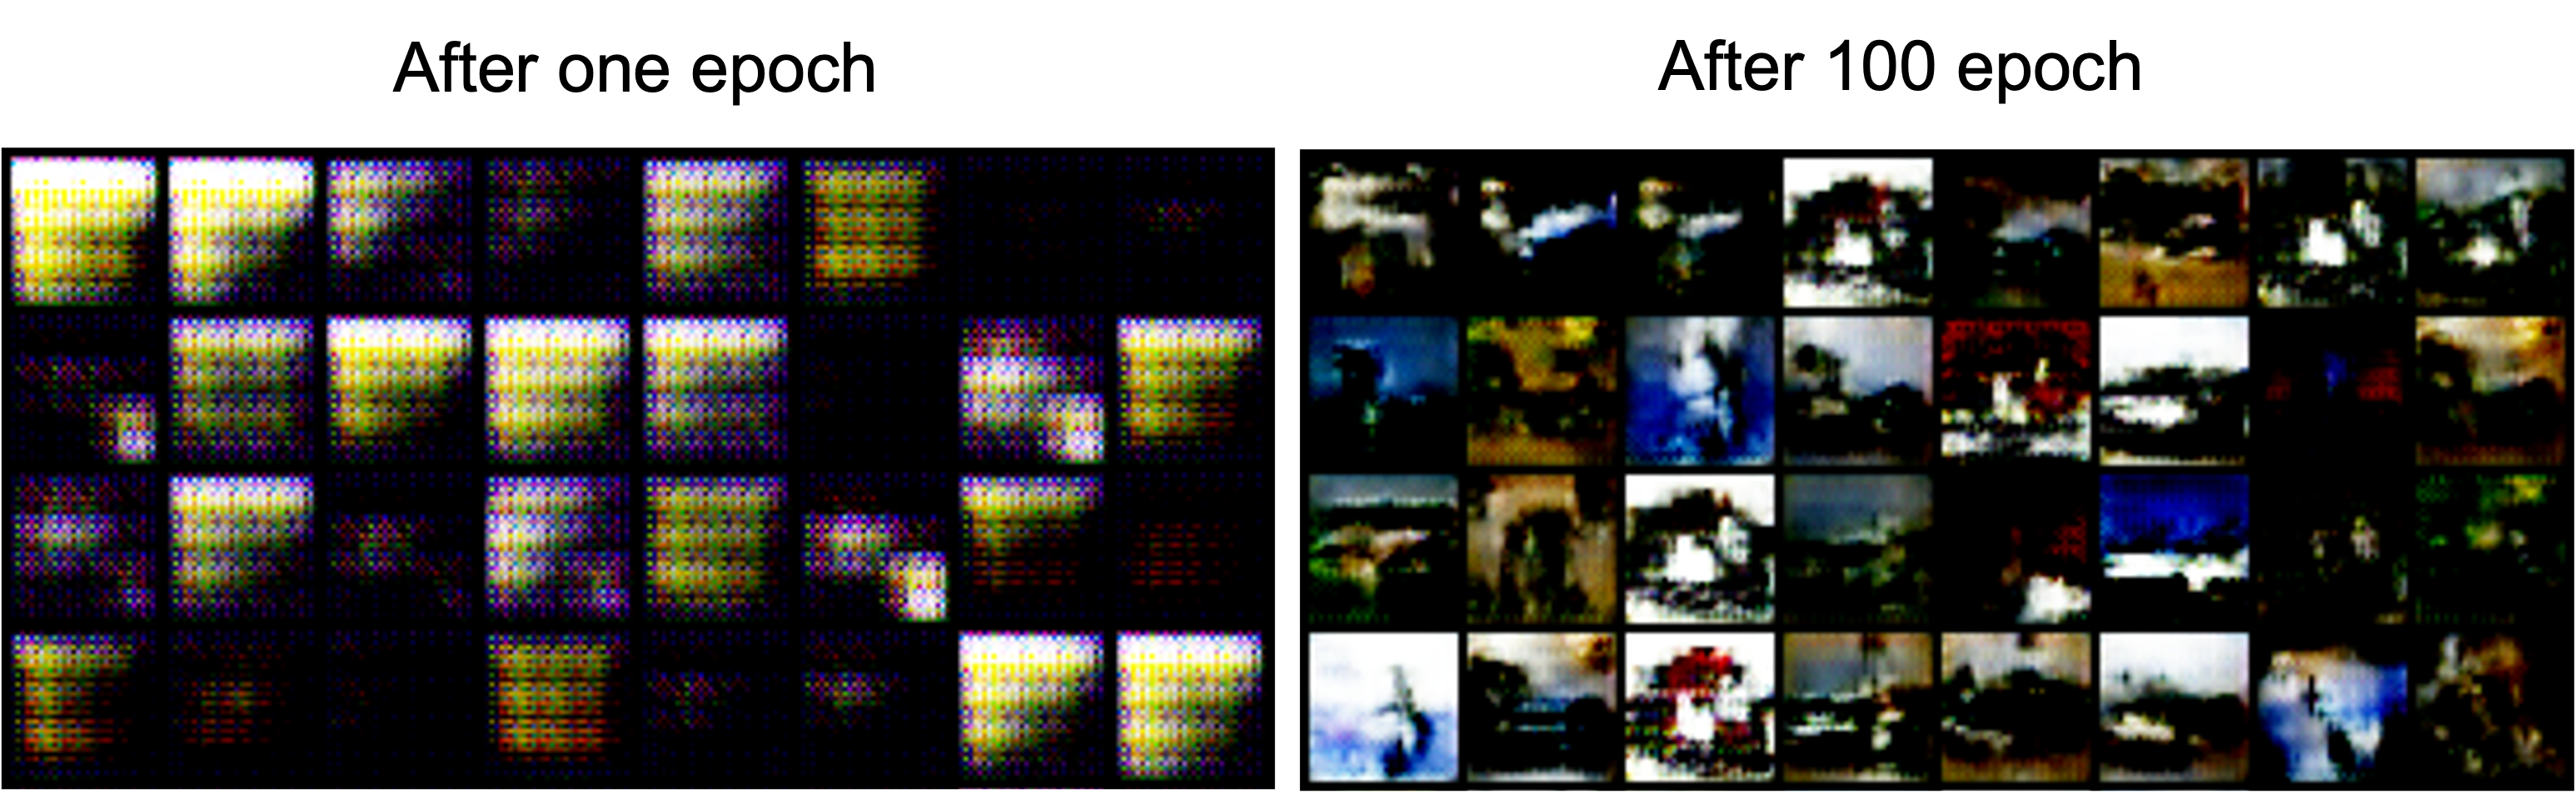
\includegraphics[scale=0.7]{AC-GAN.png}
    \label{fig:1-7}
\end{figure}


\end{itemize}
\end{solution}




\noindent\rule{7in}{2.8pt}
\end{document}


\begin{figure}[H]
\centering
    \begin{subfigure}[b]{0.45\textwidth}
    \includegraphics[scale=0.4]{HW1-1.png}
    \end{subfigure}  
    \begin{subfigure}[b]{0.45\textwidth}
    \includegraphics[scale=0.4]{HW1-2.png}
    \end{subfigure}
    \caption{The left figure show the function $sin(5\pi x)$  vs. $5\pi x$. The right figure shows the function panel $SIGN(sin(5\pi x))$  vs. $5\pi x$. In each figure, the upper panel presents the $MSE loss$ as a function of training epoch. The lower panel present the fitting to ground truth data.}
    \label{fig:1-1}
\end{figure}
